%% FINDINGS %%

\section{Findings}

\subsection{Perceptions of Agents}

As shown in \autoref{tbl:perceptions}, there are four categories defined for the perceptions of conversational agents covering 11 different aspects of perception. The details of each category and aspect are discussed below.

\textbf{Perception of interaction with agent} assesses the overall interaction quality users had with the conversational agent. The three aspects for this perceptions are usability, engagement and satisfaction. \textit{Usability} captures the utilitarian component of the interaction, whether it was accurate, easy to use, efficient or helpful. Some commonly used methods to evaluate usability include the response accuracy portion of the SASSI questionnaire \cite{hone2000towards}\cmt{sassi}, or the NASA Task Load Index (NASA-TLX) \cite{hart1988development}\cmt{nasa} for cognitive workload. Questions such as "the system is easy to use" or "it is easy to understand the agent" are also used to evaluate usability. \textit{Engagement} on the other hand captures users' emotional reactions to the CA, whether they have enjoyed the conversation, or annoyed or frustrated with the interaction. Some commonly used methods to evaluate engagement include the annoyance portion of the SASSI questionnaire \cite{hone2000towards}\cmt{sassi}, and the Use Engagement Scale (UES) \cite{o2018practical}\cmt{ues}. Questions such as "I enjoyed using the system" or "I felt frustrated with the agent" are also used to evaluate engagement. Lastly, \textit{Satisfaction} captures users' overall satisfaction interacting with the agent. Questions such as "the overall assessment of conversing with the CA was satisfactory" are used to evaluate this perception.

\textbf{Perception of agent's ability} assesses the perceived capabilities of the agent. Unlike system capabilities that affect agent's performance, the perceived ability category captures perceptions of agents with equivalent system capabilities but varied conversation architecture elements. Specifically, \textit{intelligence} captures the agent's expertise and knowledge, and it is commonly administered through the Godspeed questionnaire \cite{bartneck2009measurement}\cmt{godspeed} using the set of questions related to perceived intelligence. Also survey questions such as asking users about the agent's intelligence and domain knowledge are used to evaluate perceived intelligence. \textit{Competence} takes intelligence one step further by examining the agent's ability to put its intelligence into practice. Surveys or qualitative feedback are usually used to assess if the agent is capable and competent, and whether users have confidence in the agent's ability to get the job done. Lastly, \textit{credibility} captures agent's truthfulness, benevolence, and user's confidence in CAs. Some commonly used methods to evaluate trust include the Trust Propensity Scale \cite{mayer1999effect} and the Individualized Trust Scale (ITS) \cite{wheeless1977measurement}. Questions such as "is the agent honest" and "can I trust the agent with sensitive information" are also used to evaluate trust.

\textbf{Perception of the sociability with agent} assesses the emotional connections that users have with agents. This category includes perception aspects of conversation tone, social presence and intimacy. \textit{Conversation tone} captures the affective impression of the agent's tone, such as empathy and expressiveness. Also, this aspect includes whether the tone used by the agent was perceived as friendly, polite or warm. \textit{Social presence} captures the sense of connectness and psychological distance users have with an agent. Some aspects in this category include the sense of familiarity or similarity with the agent, and whether users feel the agent behaves like them or have similar attitudes to them. The category of \textit{Intimacy} extends social presence into the realm of the quality of relationships with an agent. Some commonly used methods to assess intimacy include the set of social attraction questions from the interpersonal attraction questionnaire \cite{mccroskey1975development} and the quality of relationship inventory (QRI) \cite{pierce1997assessing}. These questionnaires include questions like "I think the agent could be a friend of mine", or "I feel we could establish a personal relationship with each other".

\textbf{Perception of agent's humanness} assesses the specifics of anthropomorphized perceptions of conversational agents. \textit{Human-likeness} captures whether the agent presented itself as natural and human-like, or artificial and machine-like. The Godspeed questionnaire \cite{bartneck2009measurement}\cmt{godspeed} set of questions related to anthropomorphism and the Ascent of Man scale \cite{kteily2015ascent} are commonly used methods to evaluate human-likeness. Survey questions with semantic scales such as "human-like / machine-like" and "artificial / natural" are also commonly used for this aspect of perception. \textit{Personality traits} captures the human characteristics that are attributes to the agent. This is commonly collected as qualitative feedback from users, commenting on whether the agent is extroverted or introverted, or the perceived personality such as likeable, funny or witty. Sometimes the Big-5 personality traits questionnaire \cite{gosling2003very} is used to map an agent's disposition on various personality dimensions.

Overall there is a good coverage of different aspects of perception based on the list of papers reviewed in our corpus. The most commonly explored aspect categories is the perception the interaction with agent, followed by the perception of agent's humanness. There are two aspects that are the least explored compared to the others relationships: competence within the perception of agent's ability, and intimacy within the perception of social connection with agent. This may be due to the controlled lab settings for the experiments, where participants are given the scenarios for interaction. This type of environment is not conducive to forming relationships with a conversational partner, as noted by Linnerman et al. in their discussions \cite{linnemann2018can}\cmt{[15]}. The same factor could impact the assessment of agent's competence, as the users may not feel like they have the expertise to assess their perceptions. 
%These factors could contribute to the reasons why competency and intimacy are not as frequently measured in experimental studies.

%% PERCEPTION ASPECTS TABLE %%

\begin{table*}[ht]
\renewcommand*{\arraystretch}{1.4}
\resizebox{\textwidth}{!}{%
\begin{tabular}{@{}p{0.17\textwidth} | p{0.12\textwidth} | p{0.20\textwidth} | >{\centering}p{0.09\textwidth} | p{0.42\textwidth} @{}}
%!{\vrule width 1.2pt} 
\Xhline{1.2pt}
\multicolumn{2}{l|}{\textbf{Perception Aspects}} & \textbf{Examples} & \textbf{No. Papers} & \textbf{Papers} 
\\ \Xhline{1.2pt}
\multirow{3}{*}{\parbox{0.17\textwidth}{Perception of \newline Interaction with Agent}}
    & Usability & accuracy, ease of use, \newline efficiency, helpfulness & 23 
    & \cite{ashktorab2019resilient}\cmt{[88]}\cite{ceha2022expressive}\cmt{[77]}\cite{chan2021kinvoices}\cmt{[74]}\cite{choi2020nobody}\cmt{[54]}\cite{cuadra2021my}\cmt{[67]}\cite{dubiel2020persuasive}\cmt{[60]}\cite{elsholz2019exploring}\cmt{[61]}\cite{haas2022keep}\cmt{[78]}\cite{habler2019effects}\cmt{[63]}\cite{healey2013relating}\cmt{[39]}\cite{hu2022polite}\cmt{[76]}\cite{huiyang2022improving}\cmt{[17]}\cite{jestin2022effects}\cmt{[81]}\cite{kim2019comparing}\cmt{[89]}\cite{kim2020can}\cmt{[24]}
    \cite{kraus2020effects}\cmt{[64]}\cite{linnemann2018can}\cmt{[15]}\cite{ma2022ask}\cmt{[29]}\cite{miehle2018exploring}\cmt{[51]}\cite{misu2011toward}\cmt{[83]}\cite{roy2021users}\cmt{[71]}\cite{spillner2021talk}\cmt{[18]}\cite{wilhelm2022keep}\cmt{[28]}
\\ \cline{2-5}
    & Engagement & enjoyment, annoyance, \newline desirable, intention to use  & 28
    & \cite{andrews2012system}\cmt{[38]}\cite{ceha2022expressive}\cmt{[77]}\cite{ceha2021can}\cmt{[57]}\cite{chan2021kinvoices}\cmt{[74]}\cite{cox2022does}\cmt{[27]}\cite{cuadra2021my}\cmt{[67]}\cite{elsholz2019exploring}\cmt{[61]}\cite{fadhil2018effect}\cmt{[52]}\cite{gnewuch2022opposing}\cmt{[20]}\cite{go2021conversational}\cmt{[80]}\cite{healey2013relating}\cmt{[39]}\cite{huiyang2022improving}\cmt{[17]}\cite{jestin2022effects}\cmt{[81]}\cite{kim2020can}\cmt{[24]}\cite{kim2019comparing}\cmt{[89]}
    \cite{lee2020hear}\cmt{[23]}\cite{linnemann2018can}\cmt{[15]}\cite{ma2022ask}\cmt{[29]}\cite{miehle2018exploring}\cmt{[51]}\cite{miyamoto2017improving}\cmt{[46]}\cite{moilanen2022measuring}\cmt{[82]}\cite{roy2021users}\cmt{[71]}\cite{spillner2021talk}\cmt{[18]}\cite{volkel2021examining}\cmt{[69]}\cite{volkel2022user}\cmt{[75]}\cite{xiao2021let}\cmt{[73]}\cite{yang2021effect}\cmt{[72]}\cite{zhu2022effects}\cmt{[26]}    
\\ \cline{2-5}
    & Satisfaction & service satisfaction, quality of interaction & 12
    & \cite{ceha2022expressive}\cmt{[77]}\cite{choi2020nobody}\cmt{[54]}\cite{diederich2019emulating}\cmt{[25]}\cite{elsholz2019exploring}\cmt{[61]}\cite{habler2019effects}\cmt{[63]}\cite{gnewuch2018faster}\cmt{[19]}\cite{hoegen2019end}\cmt{[31]}\cite{hu2022polite}\cmt{[76]}\cite{ma2022ask}\cmt{[29]}\cite{roy2021users}\cmt{[71]}\cite{wilhelm2022keep}\cmt{[28]}\cite{yang2017perceived}\cmt{[44]}
\\ \Xhline{1.2pt} 
\multirow{3}{*}{\parbox{0.16\textwidth}{Perception of Agent's Ability}}
    & Intelligence & knowledgeable, intelligent, expertise & 11
    & \cite{ashktorab2019resilient}\cmt{[88]}\cite{ceha2021can}\cmt{[57]}\cite{chan2021kinvoices}\cmt{[74]}\cite{cuadra2021my}\cmt{[67]}\cite{dubiel2020persuasive}\cmt{[60]}\cite{feijoo2021effects}\cmt{[70]}\cite{hu2021enhancing}\cmt{[56]}\cite{jeong2019exploring}\cmt{[10]}\cite{spillner2021talk}\cmt{[18]}\cite{volkel2022user}\cmt{[75]}\cite{yang2017perceived}\cmt{[44]} 
\\ \cline{2-5}
    & Competence & competent, appropriate & 6 
    & \cite{cox2022does}\cmt{[27]}\cite{kraus2020effects}\cmt{[64]}\cite{jestin2022effects}\cmt{[81]}\cite{lee2019s}\cmt{[55]}\cite{misu2011toward}\cmt{[83]}\cite{westerman2019believe}\cmt{[9]}
\\ \cline{2-5}
    & Trust & credibility, trustworthy, truthfulness, confidence & 15
    & \cite{andrews2012system}\cmt{[38]}\cite{chan2021kinvoices}\cmt{[74]}\cite{dubiel2020persuasive}\cmt{[60]}\cite{fadhil2018effect}\cmt{[52]}\cite{healey2013relating}\cmt{[39]}\cite{hoegen2019end}\cmt{[31]}\cite{huiyang2022improving}\cmt{[17]}\cite{jestin2022effects}\cmt{[81]}\cite{kraus2020effects}\cmt{[64]}\cite{lee2020hear}\cmt{[23]}\cite{linnemann2018can}\cmt{[15]}\cite{ma2022ask}\cmt{[29]}\cite{seeger2021chatbots}\cmt{[35]}\cite{tolmeijer2021female}\cmt{[62]}\cite{wilhelm2022keep}\cmt{[28]}    
\\ \Xhline{1.2pt} 
\multirow{3}{*}{\parbox{0.16\textwidth}{Perception of \newline Sociability with Agent}}
    & Conversation Tone & friendly, warm, empathetic, persuasive & 20 
    & \cite{ashktorab2019resilient}\cmt{[88]}\cite{chan2021kinvoices}\cmt{[74]}\cite{cox2022does}\cmt{[27]}\cite{cuadra2021my}\cmt{[67]}\cite{daher2020empathic}\cmt{[58]}\cite{diederich2019emulating}\cmt{[25]}\cite{dubiel2020persuasive}\cmt{[60]}\cite{healey2013relating}\cmt{[39]}\cite{hu2021enhancing}\cmt{[56]}\cite{hu2022polite}\cmt{[76]}\cite{jestin2022effects}\cmt{[81]}\cite{khooshabeh2011does}\cmt{[37]}\cite{kim2019comparing}\cmt{[89]}\cite{lee2019s}\cmt{[55]}\cite{miehle2018exploring}\cmt{[51]}
    \cite{moilanen2022measuring}\cmt{[82]}\cite{tolmeijer2021female}\cmt{[62]}\cite{yang2021effect}\cmt{[72]}\cite{yang2017perceived}\cmt{[44]}\cite{zhu2022effects}\cmt{[26]}
\\ \cline{2-5}
    & Social Presence & connectedness, familiarity, psychological distance & 18
    & \cite{ceha2022expressive}\cmt{[77]}\cite{ceha2021can}\cmt{[57]}\cite{chan2021kinvoices}\cmt{[74]}\cite{choi2020nobody}\cmt{[54]}\cite{cuadra2021my}\cmt{[67]}\cite{diederich2019emulating}\cmt{[25]}\cite{gnewuch2018faster}\cmt{[19]}\cite{gnewuch2018chatbot}\cmt{[21]}\cite{gnewuch2022opposing}\cmt{[20]}\cite{go2021conversational}\cmt{[80]}\cite{khooshabeh2011does}\cmt{[37]}\cite{kim2020can}\cmt{[24]}\cite{lee2019s}\cmt{[55]}\cite{lubis2019positive}\cmt{[43]}\cite{lubold2016effects}\cmt{[86]}
    \cite{ma2022ask}\cmt{[29]}\cite{niewiadomski2013laugh}\cmt{[85]}\cite{westerman2019believe}\cmt{[9]}    
\\ \cline{2-5}
    & Intimacy & intimate, rapport, quality of relationship & 7 
    & \cite{choi2020nobody}\cmt{[54]}\cite{khooshabeh2011does}\cmt{[37]}\cite{kim2020can}\cmt{[24]}\cite{lee2020hear}\cmt{[23]}\cite{linnemann2018can}\cmt{[15]}\cite{lubold2016effects}\cmt{[86]}\cite{westerman2019believe}\cmt{[9]}
\\ \Xhline{1.2pt}
\multirow{2}{*}{\parbox{0.16\textwidth}{Perception of Agent's Humanness}}
    & Human-likeness & human-like, natural, \newline artificial, machine-like & 20
    & \cite{ashktorab2019resilient}\cmt{[88]}\cite{ceha2021can}\cmt{[57]}\cite{chan2021kinvoices}\cmt{[74]}\cite{choi2020nobody}\cmt{[54]}\cite{cox2022does}\cmt{[27]}\cite{diederich2019emulating}\cmt{[25]}\cite{gnewuch2018faster}\cmt{[19]}\cite{haas2022keep}\cmt{[78]}\cite{hu2022polite}\cmt{[76]}\cite{jeong2019exploring}\cmt{[10]}\cite{jestin2022effects}\cmt{[81]}\cite{lubis2019positive}\cmt{[43]}\cite{ma2022ask}\cmt{[29]}\cite{misu2011toward}\cmt{[83]}\cite{niewiadomski2013laugh}\cmt{[85]}
    \cite{ouchi2019should}\cmt{[59]}\cite{seeger2021chatbots}\cmt{[35]}\cite{wester2015artificial}\cmt{[14]}\cite{westerman2019believe}\cmt{[9]}\cite{zhu2022effects}\cmt{[26]}    
\\ \cline{2-5}
    & Personality Traits & likeable, kind, witty, funny, creepy & 20
    & \cite{andrews2012system}\cmt{[38]}\cite{ceha2022expressive}\cmt{[77]}\cite{ceha2021can}\cmt{[57]}\cite{chan2021kinvoices}\cmt{[74]}\cite{cuadra2021my}\cmt{[67]}\cite{haas2022keep}\cmt{[78]}\cite{habler2019effects}\cmt{[63]}\cite{healey2013relating}\cmt{[39]}\cite{hu2022polite}\cmt{[76]}\cite{huiyang2022improving}\cmt{[17]}\cite{jeong2019exploring}\cmt{[10]}\cite{kim2019comparing}\cmt{[89]}\cite{lee2020hear}\cmt{[23]}\cite{linnemann2018can}\cmt{[15]}\cite{miehle2018exploring}\cmt{[51]}
    \cite{ouchi2019should}\cmt{[59]}\cite{volkel2021manipulating}\cmt{[68]}\cite{volkel2022user}\cmt{[75]}\cite{wester2015artificial}\cmt{[14]}\cite{zhu2022effects}\cmt{[26]} 
\\ \Xhline{1.2pt}
\end{tabular}%
}
\caption{Perception aspects}
\label{tbl:perceptions}
\end{table*}
%% CONVERSATION ARCHITECTURE ELEMENTS TABLE %%

\begin{table*}[t]

\caption{Categories of the conversation architecture elements with examples and related papers identified from our review.}
\Description{This table categorizes conversation architecture elements into four categories, provides some examples for the element, and shows the number of papers as well as references to the papers in our reviewed corpus. The first category is dialog strategy, which contains the elements of social dialog, initiative and response delay. The second category is content affectiveness, which contains the elements of affective language and humour. The third category is content style, which contains the elements of formality, alignment and elaborateness. The fourth category is speech format, which contains the elements of prosody, disfluency, and text formatting.}
\resizebox{\textwidth}{!}{
\renewcommand*{\arraystretch}{1.4}
\begin{tabular}{@{}p{0.17\textwidth} | p{0.14\textwidth} | p{0.25\textwidth} | >{\centering}p{0.09\textwidth} | p{0.34\textwidth} @{}}
\Xhline{1.2pt}
\multicolumn{2}{l|}{\textbf{Conversation Architecture Elements}} & \textbf{Examples} & \textbf{No. Papers} & \textbf{Papers}
\\ \Xhline{1.2pt}
\multirow{3}{*}{Dialog Strategy} & Social Dialog & social talk, self-disclosure  & 7
& \cite{andrews2012system}\cmt{[38]}\cite{lee2020hear}\cmt{[23]}\cite{lubold2016effects}\cmt{[86]}\cite{moilanen2022measuring}\cmt{[82]}\cite{roy2021users}\cmt{[71]}\cite{volkel2021manipulating}\cmt{[68]}\cite{volkel2022user}\cmt{[75]}
\\ \cline{2-5}

& Initiative & proactive dialogue, conversation \newline repair & 4
& \cite{ashktorab2019resilient}\cmt{[88]}\cite{cuadra2021my}\cmt{[67]}\cite{kraus2020effects}\cmt{[64]}\cite{xiao2021let}\cmt{[73]}
\\ \cline{2-5}

& Response Delay & response delay, typing indicator & 4
& \cite{gnewuch2018faster}\cmt{[19]}\cite{gnewuch2018chatbot}\cmt{[21]}\cite{gnewuch2022opposing}\cmt{[20]}\cite{seeger2021chatbots}\cmt{[35]}
\\ \Xhline{1.2pt}

\multirow{2}{*}{Content Affectiveness} & Affective Language & emotional expressions, sentiment-adaptive responses & 11
& \cite{daher2020empathic}\cmt{[58]}\cite{diederich2019emulating}\cmt{[25]}\cite{healey2013relating}\cmt{[39]}\cite{hu2022polite}\cmt{[76]}\cite{lee2019s}\cmt{[55]}\cite{lubis2019positive}\cmt{[43]}\cite{moilanen2022measuring}\cmt{[82]}\cite{seeger2021chatbots}\cmt{[35]}\cite{volkel2022user}\cmt{[75]}\cite{yang2017perceived}\cmt{[44]}\cite{zhu2022effects}\cmt{[26]}
\\ \cline{2-5}

& Humour & humorous content, jokes & 6
& \cite{ceha2021can}\cmt{[57]}\cite{go2021conversational}\cmt{[80]}\cite{khooshabeh2011does}\cmt{[37]}\cite{miyamoto2017improving}\cmt{[46]}\cite{niewiadomski2013laugh}\cmt{[85]}\cite{volkel2021manipulating}\cmt{[68]}
\\ \Xhline{1.2pt}

\multirow{3}{*}{Content Style} & Formality & formal vs. casual, honorific \newline expressions & 9
& \cite{cox2022does}\cmt{[27]}\cite{elsholz2019exploring}\cmt{[61]}\cite{habler2019effects}\cmt{[63]}\cite{jestin2022effects}\cmt{[81]}\cite{kim2019comparing}\cmt{[89]}\cite{ma2022ask}\cmt{[29]}\cite{moilanen2022measuring}\cmt{[82]}\cite{ouchi2019should}\cmt{[59]}\cite{volkel2022user}\cmt{[75]}
\\ \cline{2-5}

& Alignment & content matching, lexical \newline alignment, agreeableness & 7
& \cite{healey2013relating}\cmt{[39]}\cite{hoegen2019end}\cmt{[31]}\cite{huiyang2022improving}\cmt{[17]}\cite{linnemann2018can}\cmt{[15]}\cite{spillner2021talk}\cmt{[18]}\cite{volkel2021examining}\cmt{[69]}\cite{volkel2021manipulating}\cmt{[68]}
\\ \cline{2-5}

& Elaborateness & elaborate, concise, sentence \newline structure & 6
& \cite{haas2022keep}\cmt{[78]}\cite{miehle2018exploring}\cmt{[51]}\cite{moilanen2022measuring}\cmt{[82]}\cite{roy2021users}\cmt{[71]}\cite{volkel2021manipulating}\cmt{[68]}\cite{volkel2022user}\cmt{[75]}
\\ \Xhline{1.2pt}

\multirow{3}{*}{Speech Format} & Prosody & pitch, intonation, speech rate, \newline spoken accent & 12
& \cite{chan2021kinvoices}\cmt{[74]}\cite{choi2020nobody}\cmt{[54]}\cite{dubiel2020persuasive}\cmt{[60]}\cite{feijoo2021effects}\cmt{[70]}\cite{habler2019effects}\cmt{[63]}\cite{hu2021enhancing}\cmt{[56]}\cite{jestin2022effects}\cmt{[81]}\cite{kim2020can}\cmt{[24]}\cite{lubold2016effects}\cmt{[86]}\cite{misu2011toward}\cmt{[83]}\cite{tolmeijer2021female}\cmt{[62]}\cite{zhu2022effects}\cmt{[26]}
\\ \cline{2-5}

& Disfluency & fillers, interjections, repetitions, \newline typos & 6
& \cite{ceha2022expressive}\cmt{[77]}\cite{hu2021enhancing}\cmt{[56]}\cite{jeong2019exploring}\cmt{[10]}\cite{wester2015artificial}\cmt{[14]}\cite{westerman2019believe}\cmt{[9]}\cite{yang2021effect}\cmt{[72]}
\\ \cline{2-5}

& Text Formatting & capitalization, emoticons & 6
& \cite{fadhil2018effect}\cmt{[52]}\cite{kim2019comparing}\cmt{[89]}\cite{seeger2021chatbots}\cmt{[35]}\cite{volkel2022user}\cmt{[75]}\cite{westerman2019believe}\cmt{[9]}\cite{wilhelm2022keep}\cmt{[28]}
\\ \Xhline{1.2pt}
\end{tabular}%
}
\label{tbl:conversation_architecture}
\end{table*}

\subsection{Conversation Architecture Elements}

As shown in \autoref{tbl:conversation_architecture}, there are four categories defined for conversation architecture across 12 different elements. The details of each category and element are discussed below.

The category of \textbf{dialog strategy} refers to the approach used by a conversational agent to engage in a dialogue with a user, which includes the use of social dialogs, agent-initiated content, and adding delays to responses. Specifically, the element of \textit{social dialogue} captures non-task related conversations with the user to build social connection, such as self-disclosure \cite{lee2020hear}\cmt{[23]} and small talk like chitchats \cite{lubold2016effects, volkel2021manipulating}\cmt{[86][68]}. The element of \textit{initiative} captures utterances that are initiated by the agent without direct prompts from the user. For example, the agent is taking the initiative to proactively repair the conversation with a user \cite{ashktorab2019resilient, cuadra2021my}\cmt{[88][67]}, or actively elicit feedback from users \cite{xiao2021let}\cmt{[73]}. Lastly, \textit{response delay} refers to the tactic of deliberately delaying for a certain period of time before an agent responds to users \cite{gnewuch2018faster, gnewuch2022opposing}\cmt{[19][20]}. It is mainly used in text-based CAs alongside visual displays of typing indicators \cite{gnewuch2018chatbot}\cmt{[21]}.

\textbf{Content affectiveness} refers to the conversational agent's use of language to convey emotions or to elicit emotions from users. The architecture element of \textit{affective language} captures the injection of emotional words or phrases into the agent's utterance, such as affective expressions \cite{seeger2021chatbots, yang2017perceived, zhu2022effects}\cmt{[35][44][26]}, sentiment-adaptive responses \cite{diederich2019emulating}\cmt{[25]}, and encouraging words \cite{healey2013relating}\cmt{[39]}. The other element in this category, \textit{humour}, captures an agent's attempt to include jokes in its dialog. Several studies in our reviewed corpus have explored the effect of humour on various perceptions of agents (e.g. \cite{ceha2021can, khooshabeh2011does}\cmt{[57][37]}).

The category of \textbf{content style} refers to the variations of language used in a message aside from the content meaning of the message (i.e. how something is said). The element of \textit{formality} describes the linguistic style used by the conversational agent, whether it is formal vs. casual, such as using honorific expressions to address users \cite{ouchi2019should}\cmt{[59]}. \textit{Alignment} captures the degree that the agent aligns its utterances to the users, such as lexical alignment on the content and structural of the sentences \cite{huiyang2022improving, linnemann2018can}\cmt{[17][15]}, as well as referring and agreeing with users' utterances \cite{volkel2021examining}\cmt{[69]}. Lastly, the element of \textit{elaborateness} captures the sentence complexity and length of agents' utterances. For example, Roy et al. explored the differences in perception for variations in elaborateness such as "Cloudly, possibility of snow, high: 4, low: -10" vs "Today will be cloudy, with a high of 4 and a low of -10. Snow is predicted" \cite{roy2021users}\cmt{[71]}.

Lastly, the category of \textbf{speech format} captures the non-verbal component of a conversational agent's utterances for both text and voice modalities. \textit{Disfluency} captures 
the use of non-lexical utterances like filler words ("um, uh") \cite{hu2021enhancing, jeong2019exploring}\cmt{[56][10]}, or repetition of words within a sentence \cite{yang2021effect}\cmt{[72]}. It also includes the format of using typos \cite{westerman2019believe}\cmt{[9]} for text-based agents. For voice-based agents specifically, the element of \textit{prosody} encompasses vocal qualities like pitch \cite{habler2019effects, jestin2022effects}\cmt{[63][81]}, speech rate \cite{choi2020nobody}\cmt{[54]}, and spoken accent \cite{feijoo2021effects}\cmt{[70]}. For text-based CAs, the \textit{text formatting} element includes different formats agents uses to present information to users, such as using capitalization \cite{westerman2019believe}\cmt{[9]} or emoticons \cite{kim2019comparing, wilhelm2022keep}\cmt{[89][28]}. 

Overall there are similar number of conversation architecture elements explored across the four categories of dialog strategy, content affectiveness, content style, and speech format. As for explorations related to different modalities of agents, there is a noticeable difference in the category of speech format, where architecture elements related to voice-based agents (n=15) are explored more than text-based agents (n=7). Looking across the 12 different elements, there is good coverage of studies on the impact of affective language and prosody cues on the perceptions of agents. However, there are less studies exploring the effect of agent initiated content and response delay on the perception of agents. Specifically for the element of initiative under dialog strategy category, there is literature on conversation repairs \cite{komatani2010online, reinkemeier2022repair} and agent proactively sharing content with users \cite{dubiel2019inquisitive, zargham2022understanding}, but many of them did not not include assessments of perceptions of the CA. This may be due to the fact that the usage of agent-initiated content is relatively new, as CA interactions have historically been driven by users. As such, current research is focused on the functional aspects of agents initiating contents instead of exploring the perceptions of agents. As for response delay, there are indications that this element is under-explored in literature. Only 4 studies in our reviewed corpus used an agent with response delay, and the majority of these publications were written by the same authors.


\subsection{Relationship Between Perceptions of Agents and Conversation Architecture}

There are 183 identified relationships between perceptions of agents and conversation architecture out of the 265 explored connections that are included in our synthesized framework (\autoref{fig:heatmap_identified}). To compare the number of identified relationships vs. the explored connections in literature, \autoref{fig:heatmap_coverage} shows a side-by-side comparison between the two. The detailed analysis on the differences between explored and identified relationships are discussed in the subsections below.

While the number of papers studying CAs with voice (n=27) vs. text (n=30) modalities is not significantly different, there are some interesting patterns we found with regards to the modalities of the identified relationships between perceptions of agents and conversation architecture. Overall, we confirmed the pattern found earlier that there are more conversation architecture elements explored related to voice vs. text in the speech format category. Because there are smaller number of text-based CAs using speech format elements, we also observed significantly less number of relationships between text-based CA across all perceptions of agents. other interesting findings related to modality are discussed later in this paper.

%% Side by side comparison between coverage and identified relationships

\begin{figure*}[]
  \centering
  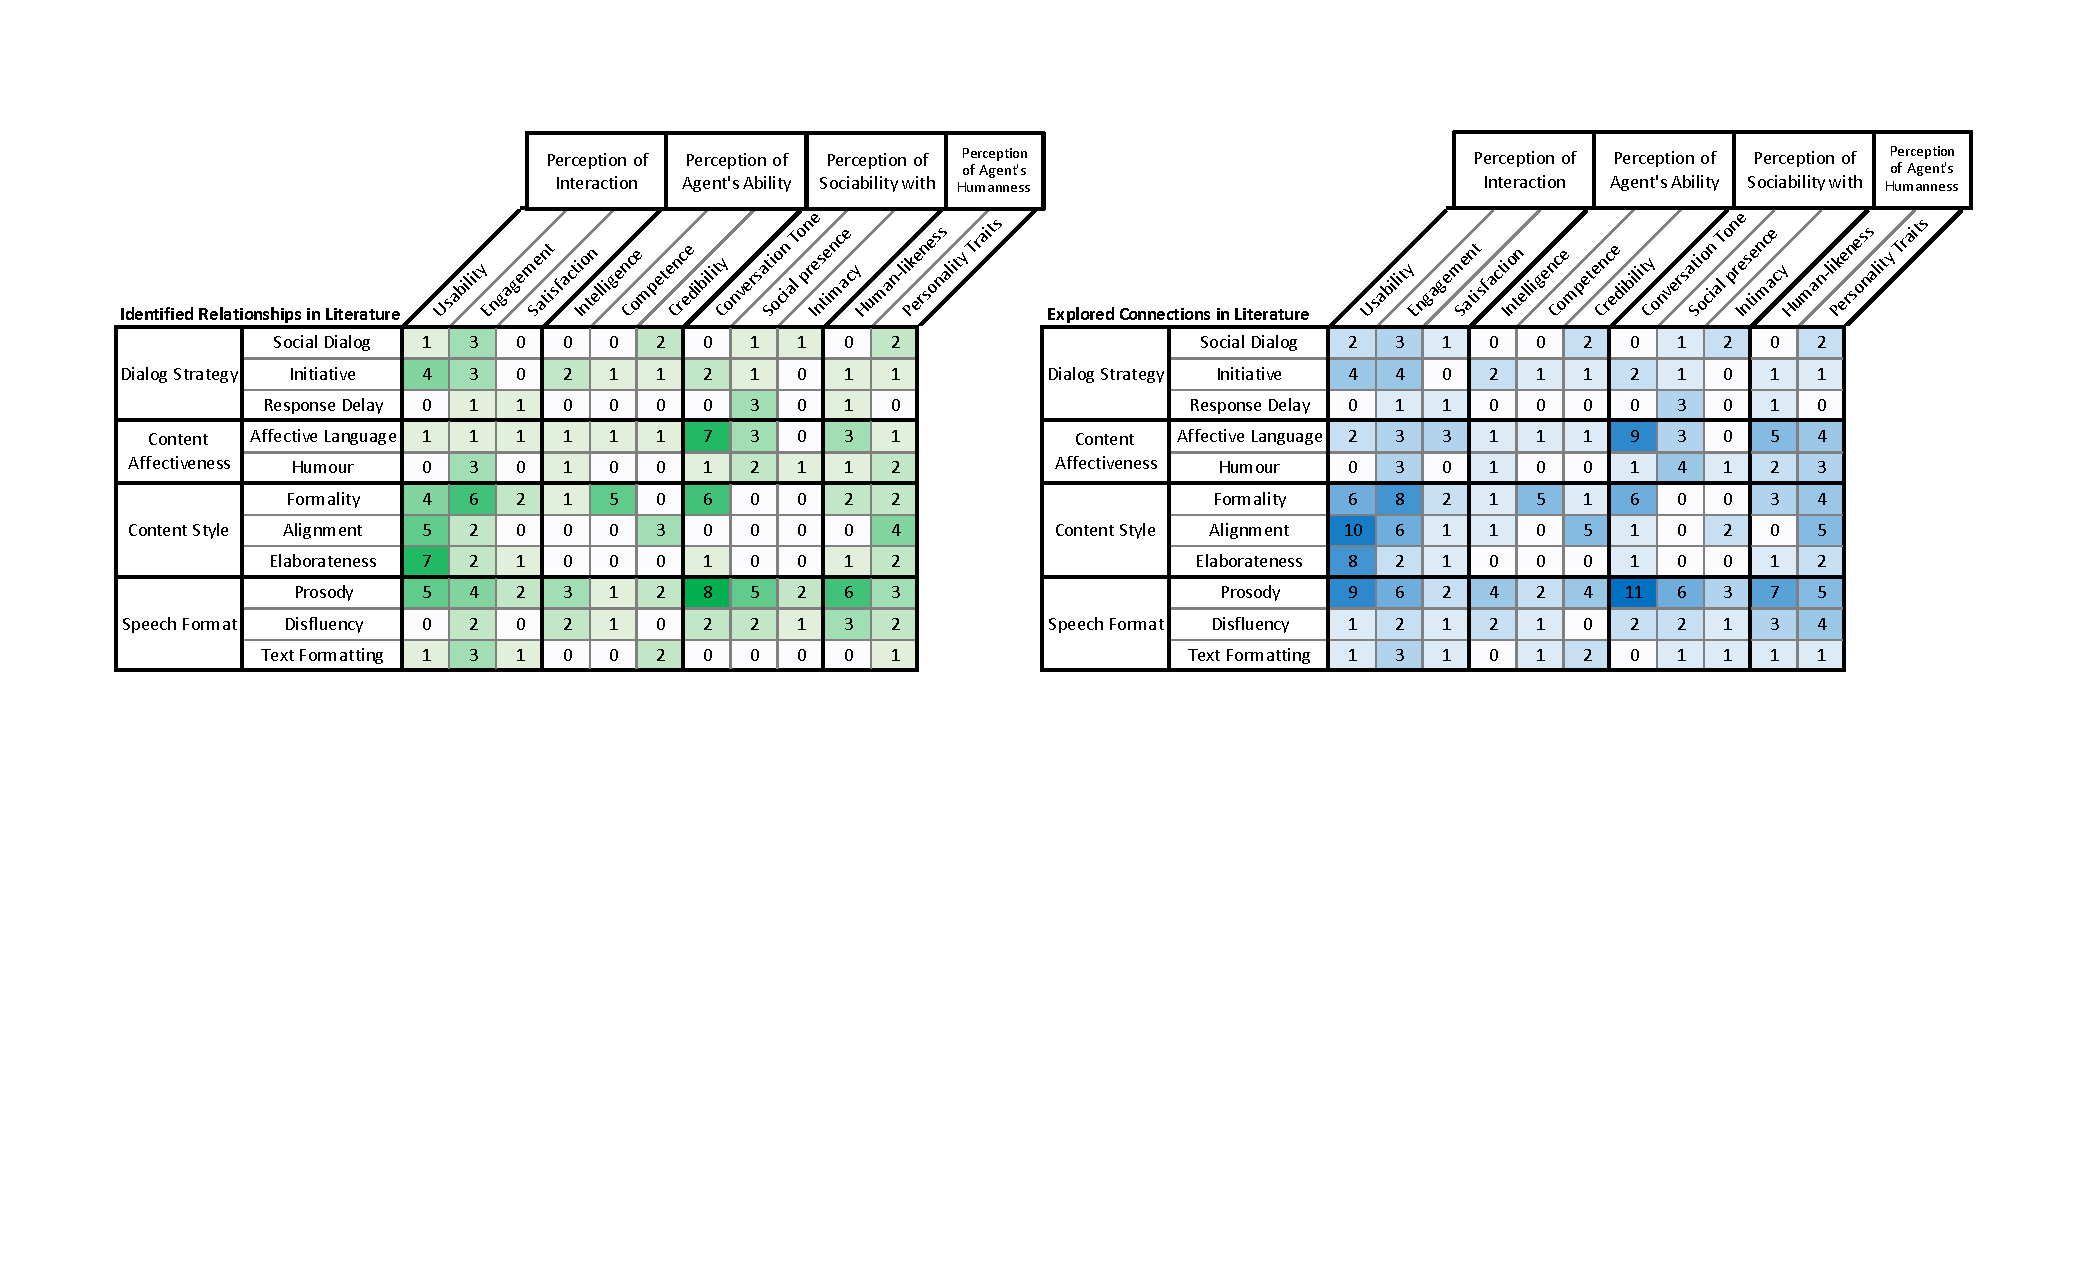
\includegraphics[width=\textwidth]{figures/fig-heatmap_coverage.pdf}
  \caption{Comparison between identified relationships and explored connections in literature}
  \Description{This figure shows a side by side comparison between the 183 identified relationships and the 265 explored connections in literature for conversation architecture elements and perceptions of agents. The visuals are shown as two heatmaps, with darker shades depicting higher number of relationships. The numbers within each cell at the interaction of a specific conversation architecture element and perception aspect outlines the number of relationships found in the reviewed corpus.}
  \label{fig:heatmap_coverage}
\end{figure*}

\subsubsection{Perception of Interaction with Agent}

The effects of conversation architecture elements on the perception of interaction with agent is the most explored connections in the corpus (n=97). Out of these explored connections, the majority of them (n=66) discovered a relationship between aspects of perception related to the perception of interaction with agent related to the studied architecture element. Looking at the difference between modalities, we noticed more voice-based agents (n=25) resulted in null relationships compared to text-based agents (n=6). The conversation architecture element of \textit{alignment} contributed the most to the null results for voice-based agents, with 9 out of 11 explored connections did not find any relationships related the perception of interaction with agents.

Across the aspects for the perception of interaction, both usability and engagement were assessed frequently in the reviewed literature, with conversation architecture having effects on these perception aspects across all architecture element categories. The aspect of satisfaction was used in some studies to evaluate perception but it is not used as often as engagement or usability. Several papers that assessed user satisfactions were conversation agents within the transaction context, especially within the customer service domain (e.g. \cite{diederich2019emulating, elsholz2019exploring, gnewuch2018faster}\cmt{[25][61][19]}).

The category of conversation architecture elements with the most identified relationships to perceptions of interaction is content style. Specifically for the element of \textit{elaborateness}, users found the use of full sentences more useful than keyword only \cite{haas2022keep, roy2021users}\cmt{[78][71]}. Otherwise, the effect of an agent's elaborateness on user's perception of interaction depends on the user's preference \cite{miehle2018exploring}\cmt{[51]}, as well as the topic of discussion \cite{haas2022keep}\cmt{[78]}. As for \textit{formality}, various studies reported significant differences in perceptions of interaction between using casual vs. formal styles. Some users experienced higher engagement with agent interacting with the casual style of the conversation \cite{cox2022does}\cmt{[27]}, while in another study users reported the formal language style as less engaging as it is boring \cite{kim2019comparing}\cmt{[89]}.

The speech format of an agent also resulted in a high number of identified relationships with the perception of interaction with CAs, with majority of the explored connections resulted in effects between the perception aspects and architecture elements. The element with the most identified relationships is \textit{prosody}. For example, studies found that a CA's expressiveness in vocal cues increased participants' engagement ratings \cite{zhu2022effects}\cmt{[26]}, and different pitches of voice affect users' perception of engagement and usability \cite{chan2021kinvoices, habler2019effects}\cmt{[74][63]}.

Dialog strategy and content affectiveness categories of conversation architecture did not have as many identified relationships with perceptions of interaction. It is worth noting the effect of using the \textit{initiative} element, as CAs that use self-initiated content are perceived as more efficient and higher quality of interaction (e.g. \cite{cuadra2021my}\cmt{[67]}). Also, some studies have discovered conflicting effects between different perception aspects of interaction for CAs using \textit{social dialog}, as users enjoyed the conversation using social talk \cite{lee2020hear, roy2021users}\cmt{[23][71]}, but perceived the CA as less efficient \cite{roy2021users}\cmt{[71]}.

\subsubsection{Perception of Agent's Ability}

The effects of conversation architecture elements on the perception of agent's ability is the least explored connection in the corpus (n=39). Out of these explored connections, the majority of them (n=30) found relationships between the studied architecture element and the perceptions of agent's ability. There are no notable differences between the text and voice modalities of CAs for either explored connections or the identified relationships.

Aspects within the perception of agent's ability had similar number of identified relationships across intelligence, competence and credibility. Our review revealed that the perceived ability of a CA is also dependent on other influencing factors in addition to conversation architecture elements. Volkel et al. \cite{kraus2020effects}\cmt{[64]} found that the perception of competence of a proactive CA is dependent on task difficulty \cite{kraus2020effects}\cmt{[64]}. Also, the perception of intelligence for an agent using fillers depended on the context of the conversation, as the filler-speaking agent was perceived as less intelligent in task-oriented conditions, but was seen as slightly more intelligent in social-oriented conditions \cite{jeong2019exploring}\cmt{[10]}.

Out of the explored conversation architecture elements, \textit{prosody} had relationships identified with aspects across the perception category of agent's ability. For example, Chan et al. \cite{chan2021kinvoices}\cmt{[74]} found that agents using kin's voices are rated as more intelligent and credible than generic voices. Also, the style of speech used by an agent affects the perception of appropriateness of tone, which is an aspect of the perceived competence of an agent \cite{misu2011toward}\cmt{[83]}. Different content styles of \textit{formality} also impacts the perceived competence of an agent \cite{cox2022does, jestin2022effects}\cmt{[27][81]}. Specifically related to perceived credibility of an agent, being \textit{lexically aligned} with the user resulted improved the rating of trustworthiness of an agent \cite{hoegen2019end, linnemann2018can}\cmt{[31][15]}. There were mixed results on the use of emoticons within the \textit{text formatting} element. One study found the chatbot using emoticons as less trustworthy \cite{wilhelm2022keep}\cmt{[28]}, while another study found that users assigned higher scores for confidence to the agent using emojis \cite{fadhil2018effect}\cmt{[52]}. 

There are several conversation architecture elements with little to no explorations to the perception of agent's ability. Specifically, both categories of dialog strategy and content affectiveness are minimally explored in our reviewed corpus, with no explored connections with \textit{response delay} and only one or two connections explored for \textit{social dialog} and \textit{humour}. While the content style category had coverage in some aspects of perceived abilities, it is worth noting that \textit{elaborateness} did not have any explored connections with perceived ability of agents. Further research in these areas is needed to fill these gaps in understanding.


\subsubsection{Perception of Sociability with Agent}

The perception of agent's humanness is the second most explored category within our reviewed corpus (n=64), with majority of the connections identified relationship between the studied conversation architecture elements and the anthropomorphized perceptions of agent (n=49). Interestingly, studies explored more perceptions of sociability with agent related to voice-based CAs (n=40) compared to text-based CAs (n=24), potentially due to the assumption that interactions with text-based agents are perceived as less personal and more formal \cite{kocielnik2018designing}. There are some mixed results for voice-based CAs, as 12 out of the 28 connections did not find any significant results. Drilling down to the specific elements, we noticed that the use of \textit{alignment} in voice-based agents did not effect the perception of sociability with agent \cite{healey2013relating, linnemann2018can}\cmt{[39][15]}. We didn't have data on text-based agents' perceived social connections with users to compare with voice-based agents, as the studies using alignment and text modality in our corpus did not assess this aspect category of perception.

Across the aspects in this perception category, conversation tone had the most number of identified relationship (n=27) with the perceived social connection with CAs, followed by the aspect of social presence (n=17). There are only 5 relationships found that are linked to the perception aspect of intimacy. One reason for this is half of the explored connections did not have any effect on the perception of sociability with agent, such as the use of capitalization \cite{westerman2019believe}\cmt{[9]}, lexical alignment \cite{linnemann2018can}\cmt{[15]}, or social talk \cite{lubold2016effects}\cmt{[86]}. For the perception aspect of social presence, we noticed a gap in the exploration of conversation architecture elements of formality, alignment, and elaborateness in the content style category, as there are no papers explored at this intersection.

Looking at the different categories of conversation architecture elements, the heatmap (\autoref{fig:heatmap_identified}) shows that there are not many relationships in content style category that are related to the perceived sociability with CAs in general, with most of the discovered effects concentrated at the intersection of \textit{formality} and conversation tone. Studies have found that CAs using casual style of conversation are perceived as warm, empathetic and friendly \cite{jestin2022effects, kim2019comparing}\cmt{[81][89]}, while CAs using formal style of conversation are perceived as polite but lacks empathy \cite{cox2022does}\cmt{[27]}. The rest of the architecture elements and perception aspects of sociability are minimally explored in literature, which indicates the need for more research in this area.

There are a few specific conversation architecture elements that had more identified relationships with perceptions of sociability with agent. Specifically, CAs using of \textit{affective language} were perceived to be more empathetic \cite{daher2020empathic, diederich2019emulating, yang2017perceived}\cmt{[58][25][44]} and emotionally expressive \cite{zhu2022effects}\cmt{[26]}, as well as being more emotional connected with their users \cite{lee2019s, lubis2019positive}\cmt{[55][43]}. Also, different variations of a voice-based CA's \textit{prosody} have effects on the perceived sociability with agent, such as an agent using expressive prosody is assessed as more intimate and more similar with the user \cite{kim2020can}\cmt{[24]}. Lastly, the conversation architecture element of \textit{humour} has identified relationships across the social connection category of perception. Clark et al. \cite{clark2019makes} found that humour is an important conversational characteristic for human-human interactions, but viewed as a novelty feature for human-agent conversations. However, in our review we found that humor has effects on human-agent relationships, as humorous agents are rated as more friendly, intimate, and similar by users compared to non-humorous agents \cite{go2021conversational, khooshabeh2011does}\cmt{[80][37]}. 


\subsubsection{Perception of Agent's Humanness}

There are 55 explored connections between conversation architecture elements and the perception of sociability with agents, with majority of them (n=38) finding identified relationships in literature. There are significantly more explorations for voice-based agents (n=39) as compared to text-based agents (n=16). Previous studies have found that modality may have an effect on the perception of humanness, as voice-based agents are perceived as more human-like as compared to text-based agents \cite{cho2019effects}. Out of the 39 explored connections for voice-based agents, 14 of them did not result in any relationships. This is especially evident in the architecture element of \textit{affective language} for voice-based agents, as most of the connections resulted in null relationships. For example, when comparing the ratings of human-likeness or likeability for a speech agent employing expressive words to the one not using any, Zhu et al \cite{zhu2022effects}\cmt{[26]} were unable to detect any statistically significant differences in both of the observation study and interaction study.

Across the aspects in this perception category, both human-likeness and personality traits have relationships with almost all the conversation architecture elements. Specifically for the use of \textit{prosody} elements, our review found some opposing effects on the perception of the agent's humanness. In the case of Chan et al's study \cite{chan2021kinvoices}\cmt{[74]}, participated rated the agent using kin voices as significantly more likeable compared to the generic voices, but it was perceived as eerie. This may be a warning indicator to watch out for the uncanny valley effect \cite{mori2012uncanny} and advise CA designers to carefully select conversation architecture elements to elicit anthropomorphized perceptions.

There are a few notable conversation architecture elements related to the perceived humanness of conversational agents. The use of \textit{prosody} such as varying pitch, intonation and speech rate has more identified relationships with the perceived personality traits of an agent as compared to the perceived human-likeness, especially on the aspect of likeability \cite{choi2020nobody, jestin2022effects, misu2011toward}\cmt{[54][81][83]}. For the architecture elements of \textit{disfluency}, the type of impact on the perception of humanness depended on the context of the conversation. Studies have found that participants perceived the filler-condition agent as more likeable in the social-oriented situation, but did not find the same effect in task-oriented situations \cite{jeong2019exploring, wester2015artificial}\cmt{[10][14]}. The use of \textit{alignment} in an agent had a number of identified relationships with the perception of personality traits, with some studies finding CAs that are lexically aligned with a user are more likeable \cite{huiyang2022improving, linnemann2018can}\cmt{[17][15]}. 